\documentclass[border=12pt]{standalone}
\def\pgfsysdriver{pgfsys-dvisvgm.def}
\usepackage[dvisvgm]{xcolor}
\usepackage{xeCJK}
\setCJKmainfont{HaranoAjiGothic-Regular.otf}[BoldFont=HaranoAjiGothic-Bold.otf]
\setCJKsansfont{HaranoAjiGothic-Regular.otf}[BoldFont=HaranoAjiGothic-Bold.otf]
\usepackage{amsmath,amssymb,tikz,lmodern}
\usetikzlibrary{arrows.meta,positioning,calc}
\renewcommand{\familydefault}{\sfdefault}
\definecolor{ink}{HTML}{25322F}
\definecolor{green}{HTML}{246657}
\definecolor{tint}{HTML}{EEF4F0}
\definecolor{soft}{HTML}{C6D2CC}
\definecolor{muted}{HTML}{52615B}
\newif\ifJapanese
\newcommand{\Tx}[2]{\ifJapanese #1\else #2\fi}
\newcommand{\heading}[3]{{\color{green}\bfseries #1\quad\Tx{#2}{#3}}\\[5pt]}
\newcommand{\Var}{\operatorname{Var}}
\newcommand{\Frac}{\operatorname{Frac}}
\newcommand{\C}{\mathbb C}
\newcommand{\refurl}[2]{\special{dvisvgm:raw <a xlink:href="#1" target="_blank" rel="noopener noreferrer">}{\setlength{\fboxsep}{0pt}\colorbox{white}{\color{green}\underline{\strut #2}}}\special{dvisvgm:raw </a>}}
\newcommand{\R}[2]{\refurl{\csname source#1\endcsname}{#2}}
\tikzset{
 card/.style={draw=soft,fill=white,rounded corners=2pt,align=left,text=ink,font=\fontsize{10.5}{14}\selectfont,inner xsep=12pt,inner ysep=11pt,text width=14.4cm},
 result/.style={card,draw=green,fill=tint,line width=.9pt},
 reason/.style={align=left,text=muted,font=\fontsize{9}{12}\selectfont,inner sep=0pt,text width=12.7cm},
 edge/.style={-{Stealth[length=2.4mm]},draw=green,line width=1pt}
}
\newcommand{\flow}[3]{
 \coordinate (#2-from) at ($(#1.south)+(-6.9,0)$);
 \coordinate (#2-to) at ($(#2.north)+(-6.9,0)$);
 \draw[edge] (#2-from)--(#2-to);
 \node[reason,anchor=west] at ($(#2-from)!.5!(#2-to)+(.55,0)$) {#3};
}

\Japanesefalse
\expandafter\def\csname sourceWV\endcsname{https://github.com/openai/math/blob/fd4aeeb2ee4fc729c18d98444fed42fd0529eeeb/preprints/Logarithmic-Kodaira-dimension-and-whole-fiber-variation-September-26-2026/paper.pdf}
\expandafter\def\csname sourceOI\endcsname{https://github.com/openai/math/blob/fd4aeeb2ee4fc729c18d98444fed42fd0529eeeb/preprints/Orbifold-and-logarithmic-Iitaka-subadditivity-September-26-2026/paper.pdf}
\expandafter\def\csname sourcePH\endcsname{https://github.com/openai/math/blob/fd4aeeb2ee4fc729c18d98444fed42fd0529eeeb/preprints/Projective-Hodge-lines-and-ordinary-Iitaka-subadditivity-September-27-2026/paper.pdf}
\expandafter\def\csname sourceRA\endcsname{https://github.com/openai/math/blob/fd4aeeb2ee4fc729c18d98444fed42fd0529eeeb/preprints/The-reverse-logarithmic-Kodaira-inequality-and-additivity-September-26-2026/paper.pdf}
\expandafter\def\csname sourceLA\endcsname{https://github.com/openai/math/blob/adc7f1241b42e322a6451854ab7e4b4c146bf78a/preprints/Log-abundance-in-characteristic-zero-September-24-2026/paper.pdf}
\expandafter\def\csname sourceFuj\endcsname{https://www.math.kyoto-u.ac.jp/~fujino/weak-posi11.pdf}
\expandafter\def\csname sourceDel\endcsname{https://www.numdam.org/item/PMIHES_1971__40__5_0.pdf}
\expandafter\def\csname sourceDHP\endcsname{https://arxiv.org/pdf/1012.0493v2}
\expandafter\def\csname sourcePT\endcsname{https://arxiv.org/pdf/1409.5504v1}
\expandafter\def\csname sourceBCHM\endcsname{https://arxiv.org/pdf/math/0610203v2}
\expandafter\def\csname sourceKP\endcsname{https://sites.math.washington.edu/~kovacs/2013/papers/Kovacs_Patakfalvi__Projectivity.pdf}
\expandafter\def\csname sourceHan\endcsname{https://doi.org/10.1007/BF01394338}
\expandafter\def\csname sourceSGA1\endcsname{https://arxiv.org/abs/math/0206203v2}
\expandafter\def\csname sourceLan\endcsname{https://arxiv.org/pdf/2005.09690v3}
\expandafter\def\csname sourceBDPP\endcsname{https://arxiv.org/pdf/math/0405285v1}
\expandafter\def\csname sourceTaj\endcsname{https://arxiv.org/pdf/2005.01025v4}
\begin{document}
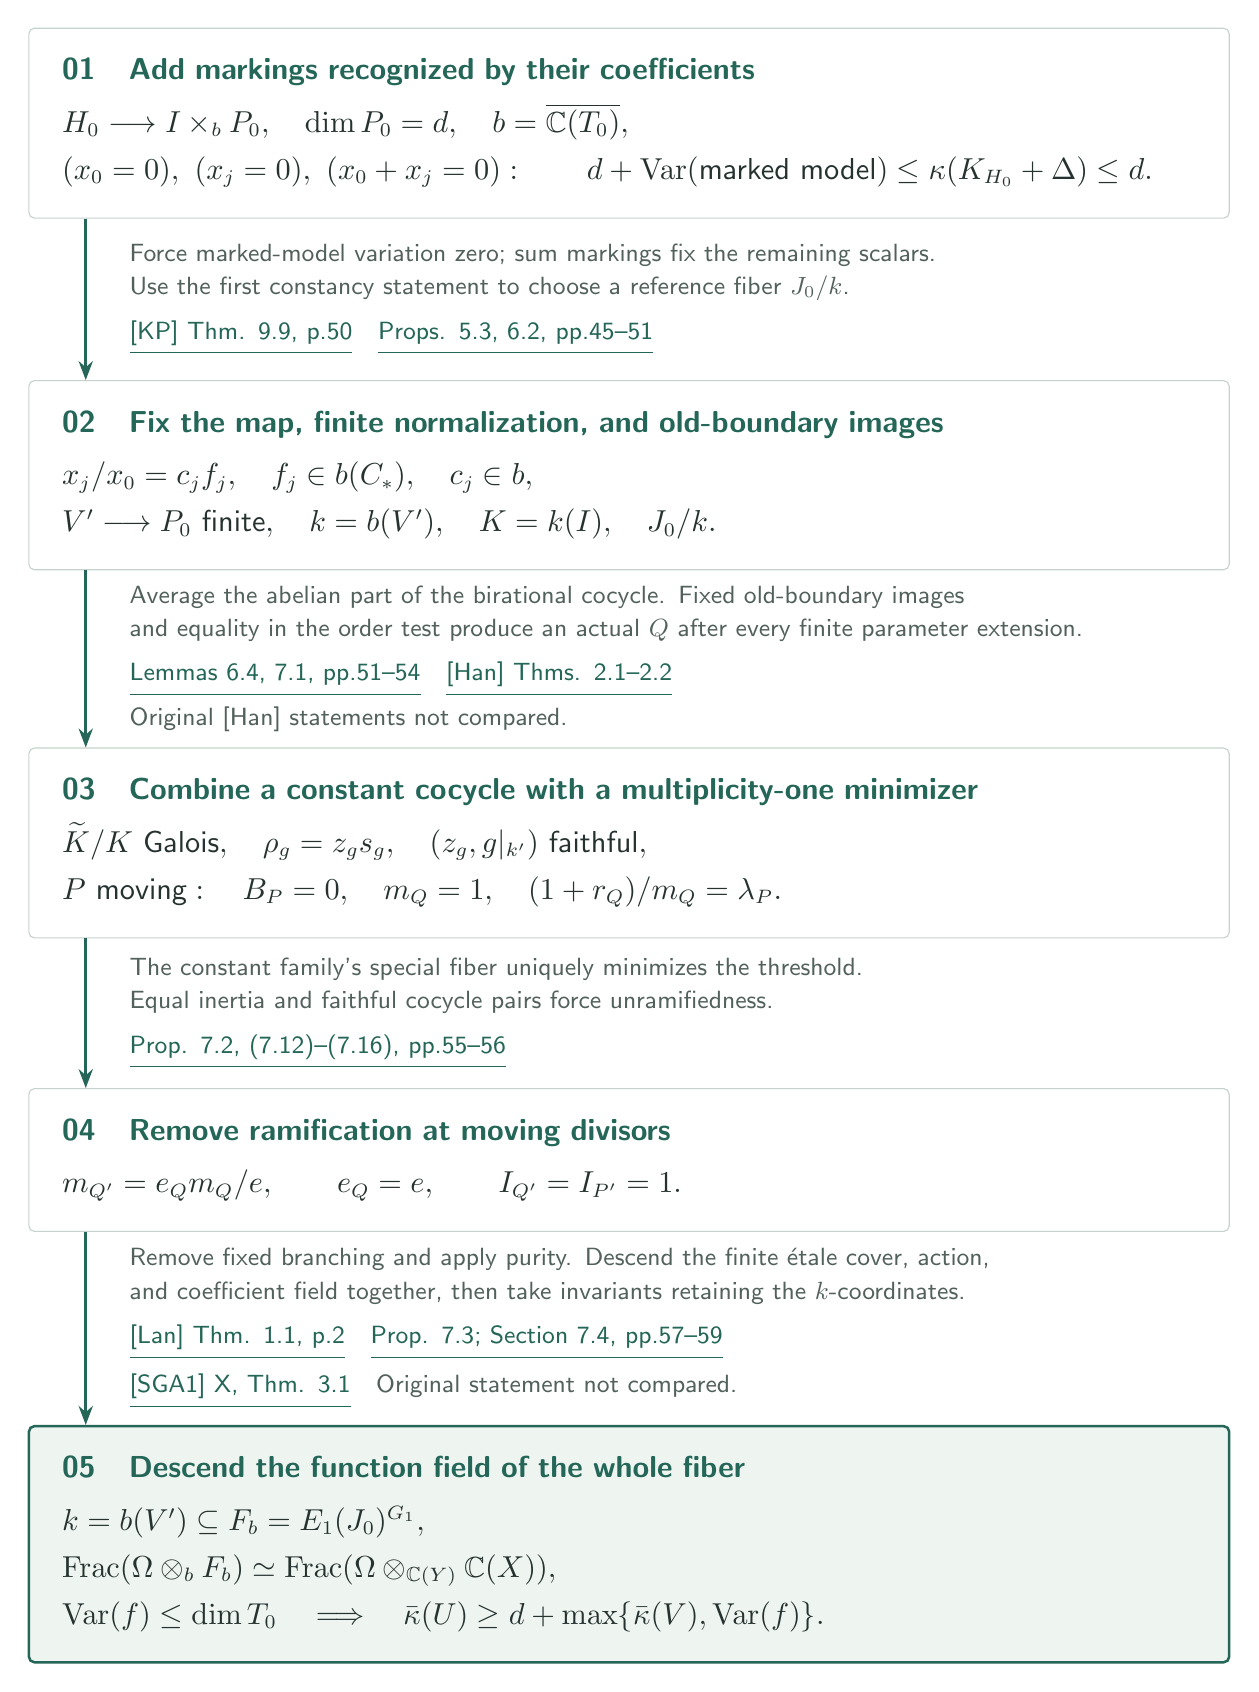
\begin{tikzpicture}
\node[card] (mark) {\heading{01}{係数で識別できるmarkingを加える}{Add markings recognized by their coefficients}
$H_0\longrightarrow I\times_bP_0,\quad \dim P_0=d,\quad b=\overline{\C(T_0)},$\\[3pt]
$(x_0=0),\ (x_j=0),\ (x_0+x_j=0):\qquad
 d+\Var(\text{marked model})\le\kappa(K_{H_0}+\Delta)\le d.$};
\node[card,below=2.05cm of mark] (base) {\heading{02}{写像・有限正規化・旧境界の像を固定する}{Fix the map, finite normalization, and old-boundary images}
$x_j/x_0=c_jf_j,\quad f_j\in b(C_*),\quad c_j\in b,$\\[3pt]
$V'\longrightarrow P_0\ \text{finite},\quad k=b(V'),\quad K=k(I),\quad J_0/k.$};
\flow{mark}{base}{\Tx{marked modelのvariationを0にし、和のmarkingで残る定数を固定する。\\最初のconstancyからreference fiber $J_0/k$ を選ぶ。}{Force marked-model variation zero; sum markings fix the remaining scalars.\\Use the first constancy statement to choose a reference fiber $J_0/k$.}\\[4pt]
\R{KP}{[KP] Thm. 9.9, p.50}\quad\R{WV}{Props. 5.3, 6.2, pp.45--51}}
\node[card,below=2.25cm of base] (two) {\heading{03}{定数cocycleとmultiplicity-one最小化因子を揃える}{Combine a constant cocycle with a multiplicity-one minimizer}
$\widetilde K/K\ \text{Galois},\quad \rho_g=z_gs_g,\quad(z_g,g|_{k'})\ \text{faithful},$\\[3pt]
$P\ \Tx{\text{moving}}{\text{moving}}:\quad B_P=0,\quad m_Q=1,\quad (1+r_Q)/m_Q=\lambda_P.$};
\flow{base}{two}{\Tx{双有理群のabelian部分でcocycleを平均する。旧境界像の固定性と\\位数の等号は、任意の有限parameter拡大後にも実際の $Q$ を与える。}{Average the abelian part of the birational cocycle. Fixed old-boundary images\\and equality in the order test produce an actual $Q$ after every finite parameter extension.}\\[4pt]
\R{WV}{Lemmas 6.4, 7.1, pp.51--54}\quad\R{Han}{[Han] Thms. 2.1--2.2}\\[3pt]
\Tx{[Han]の原典記述は未照合。}{Original [Han] statements not compared.}}
\node[card,below=1.9cm of two] (inertia) {\heading{04}{動く因子上の分岐を消す}{Remove ramification at moving divisors}
$m_{Q'}=e_Qm_Q/e,\qquad e_Q=e,\qquad I_{Q'}=I_{P'}=1.$};
\flow{two}{inertia}{\Tx{定数族のspecial fiberは閾値の一意な最小化因子。\\慣性の一致とcocycleのfaithfulnessが非分岐性を強制する。}{The constant family's special fiber uniquely minimizes the threshold.\\Equal inertia and faithful cocycle pairs force unramifiedness.}\\[4pt]
\R{WV}{Prop. 7.2, (7.12)--(7.16), pp.55--56}}
\node[result,below=2.45cm of inertia] (whole) {\heading{05}{全ファイバーの関数体を降下する}{Descend the function field of the whole fiber}
$k=b(V')\subseteq F_b=E_1(J_0)^{G_1},$\\[3pt]
$\Frac(\Omega\otimes_bF_b)\simeq\Frac(\Omega\otimes_{\C(Y)}\C(X)),$\\[3pt]
$\Var(f)\le\dim T_0\quad\Longrightarrow\quad\bar\kappa(U)\ge d+\max\{\bar\kappa(V),\Var(f)\}.$};
\flow{inertia}{whole}{\Tx{固定分岐を除きpurityを適用。有限étale被覆・群作用・係数体を\\同時に降下し、不変式を取る。飯高底の $k$ 座標を保持する。}{Remove fixed branching and apply purity. Descend the finite étale cover, action,\\and coefficient field together, then take invariants retaining the $k$-coordinates.}\\[4pt]
\R{Lan}{[Lan] Thm. 1.1, p.2}\quad\R{WV}{Prop. 7.3; Section 7.4, pp.57--59}\\[3pt]
\R{SGA1}{[SGA1] X, Thm. 3.1}\quad\Tx{原典記述は未照合。}{Original statement not compared.}}
\end{tikzpicture}

\end{document}
